\documentclass[10pt]{article}
\usepackage[polish]{babel}
\usepackage[utf8]{inputenc}
\usepackage[T1]{fontenc}
\usepackage{amsmath}
\usepackage{amsfonts}
\usepackage{amssymb}
\usepackage[version=4]{mhchem}
\usepackage{stmaryrd}
\usepackage{graphicx}
\usepackage[export]{adjustbox}
\graphicspath{ {./images/} }

\title{LIGA MATEMATYCZNA im. Zdzisława Matuskiego \\
 LISTOPAD 2018 \\
 GIMNAZJUM }

\author{}
\date{}


\begin{document}
\maketitle
(klasa VII i VIII szkoły podstawowej, klasa III gimnazjum)

\section*{ZADANIE 1.}
Czy istnieje trójkąt prostokątny mający boki o długościach całkowitych i obwód równy 2019?

\section*{ZADANIE 2.}
Wykaż, że liczba

\[
\frac{n^{5}}{120}-\frac{n^{3}}{24}+\frac{n}{30}
\]

jest całkowita dla każdej liczby całkowitej \(n\).

\section*{ZADANIE 3.}
Wyznacz wszystkie pary liczb całkowitych dodatnich \((x, y)\) o następujących własnościach:

\[
x+y=240 \quad \text { oraz } \quad \operatorname{NWD}\{x, y\}=30
\]

\section*{ZADANIE 4.}
Ile jest liczb trzycyfrowych podzielnych przez 9 mających następującą własność: suma cyfr ilorazu tej liczby przez 9 jest o 9 mniejsza od sumy jej cyfr?

\section*{ZADANIE 5.}
Sześciokąt mający wszystkie kąty wewnętrzne tej samej miary wpisano w trójkąt równoboczny o boku o długości 7. Wyznacz długości boków \(x, y, z\).\\
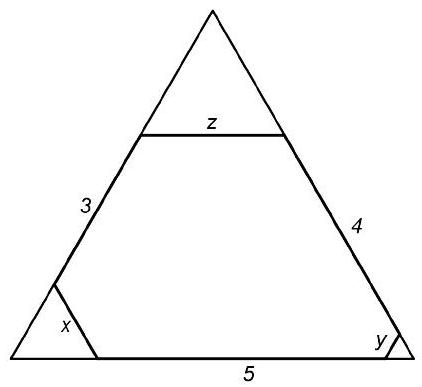
\includegraphics[max width=\textwidth, center]{2024_11_21_b9301f47f75104ae1ce5g-1}


\end{document}